\documentclass[../gruppenarbeit_1.tex]{subfiles}

% definition für mengendiagramme
\def\firstcircle{(0,0) circle (1.5cm)}
\def\secondcircle{(0:2cm) circle (1.5cm)}

\colorlet{circle edge}{blue!50}
\colorlet{circle area}{blue!20}

\tikzset{filled/.style={fill=circle area, draw=circle edge, thick},
    outline/.style={draw=circle edge, thick}}
% definition für mengendiagramme

\subsection{Einführung}

Mit Mengen lassen sich Objekte genau beschreiben und vergleichen. \\
Eine Menge ist eine Zusammenfassung, von bestimmten wohlunterscheidbaren 
Elemenenten die zu einem ganzen zusammengeführt werden.\\

\begin{itemize}
    \item Mengen sind Objekte worüber wir Aussagen machen
    \item Mengen sind wohlunterscheidbare Elemente die zu einem ganzen zusammengeführ werden
    \item Mengen sind Objekte unseres Denkens / Anschauung
\end{itemize}

$x \in M$
x ist ein Element von M

$x \notin M$
x ist kein Element von M

$\varnothing = \{\}$
Leere Menge

Ein Objekt ist entweder Element einer Menge ($\in$) oder nicht ($\notin$).

M := \{a,b,c\}
ist die Menge M, welche aus den Elementen a b c besteht

M := \{a,a,b,c\}
is keine Menge. Dasselbe Element soll nicht mehrmals vorkommen

\subsubsection{Definition von Mengen}

\def\arraystretch{1.5}
\begin{table}[ht]
\begin{tabular}[t]{lll}
    \hline
    Kürzel & Definition\\
    \hline
    $A, B$ & Mengen\\
    $a, b$ & Elemente einer Menge\\
    $x \in M$ & x ist ein Element von M\\
    $x \notin M$ & x ist kein Element von M\\
    $\varnothing = \{\}$ & Leere Menge $x$\\
    \hline
\end{tabular}
\end{table}

\begin{itemize}
  \item $M := \{a,b,c\}$: ist die Menge M, welche aus den Elementen a b c besteht
  \item $M := \{a,a,b,c\}$: is keine Menge. Dasselbe Element soll nicht 
  mehrmals vorkommen
\end{itemize}

Elemente einer Menge müssen nicht vom selben Typ sein:

$A := \{Tiger, Pi, BMW, 2+3=5\}$
\vspace{5mm}

Menge $A$ und Menge $B$ sind identisch $(A=B)$, wenn sie die selben Elemente enthalten.

$A=B : \iff \forall x : (x \in A \iff x \in B)$
\vspace{5mm}

Wenn A nicht gleich B: $A \ne B$

\subsection{Verschiedene Arten der Darstellung}

\subsubsection{Darstellung von Mengen}

\textbf{Aufzählende Form}:\\
$A := \{0,1,2,3\}$
\vspace{5mm}

\textbf{Beschreibende Form}:\\
Die Menge A aller x mit der Eigenschaft $P(x)$.\\
\vspace{5mm}

\textbf{Mathematisch Formal}:\\
$A := \{x | P(x)\}$

\begin{align}
\fbox{\begin{minipage}{11.8cm}
  \textbf{Beispiel}: Die Menge A aller natürlichen, ungeraden Zahlen 
  kleiner 10.\\
  $A := \{n | n \in \mathbb{N} \wedge n < 10 (\exists k \in \mathbb{N} : n = 2k-1)\}$
\end{minipage}}
\end{align}

\newpage

\textbf{Venn-Diagramm zur Grafischen Darstellung}:\\
$A : \{a,b,c,d\}$\\

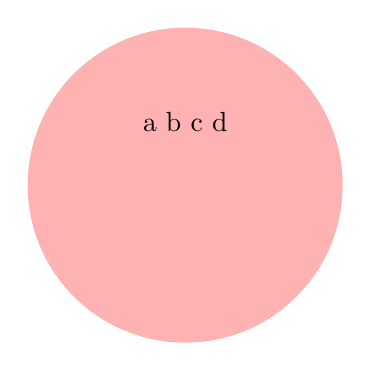
\begin{tikzpicture}
  \begin{scope}[blend group=soft light]
      \fill[red!30!white]   ( 90:1.2) circle (2);
  \end{scope}
  \node at ( 90:2)    {a b c d};
\end{tikzpicture}

\subsection{Wichtige Zahlenmengen}

\def\arraystretch{1.5}
\begin{table}[ht]
\begin{tabular}[t]{ll}
\hline
  Kürzel & Definition\\
\hline
  $\mathbb{N}$ & $\{0,1,2,3,4,5,6,...\}$\\
   & Die Menge der natürlichen Zahlen\\
  $\mathbb{Z}$ & $\{-3,-2,-1,0,1,2,3,...\}$\\
   & Die Menge der ganzen Zahlen\\
  $\mathbb{Q}$ & $\{m/n | m \in \mathbb{Z} \wedge n \in \mathbb{N} \wedge n \ne 0\}$\\
   & Die Menge der rationalen Zahlen\\
  $\mathbb{R}$ & $\{x | x ist als endlicher oder unendlicher Dezimalbruch darstellbar\}$\\
   & Die Menge der reellen Zahlen\\   
  $\mathbb{C}$ & $\{x+yi | x,y \in \mathbb{R} \wedge i := \sqrt{-1}\}$\\
   & Die Menge der komplexen Zahlen\\
\hline
\end{tabular}
\end{table}

\subsection{Teilmengen / Obermengen}

$x \in A \rightarrow x \in B$\\
$A \subseteq B$ und sagen A ist eine Teilmenge von B und B ist eine Obermenge 
von A.

Wenn $A \ne B, A \subset B$ oder $A \subsetneq B$ also eine echte Teilmenge 
oder echte Obermenge.\\

\newpage

Richtig:\\
$\{1,2,3\} \subset \{1,2,3,4,5\}$\\
$\{x,y,z\} \subseteq \{x,y,z\}$\\
\\
Falsch:\\
$\{x,y,z\} \subset \{x,y,z\}$
\vspace{5mm}

Eine Teilmenge ist gleichbedeutend mit Untermenge.\\
\\
Mächtigkeit (Kardinalität) ist die Anzahl der Elemente einer Menge und wird so dargestellt: $|A|$\\

\begin{align}
\fbox{\begin{minipage}{11.8cm}
  \textbf{Beispiel}: $A := \{a,b,c,d,e,....,y,z\}$\\
  Die Menge der kleinen Buchstaben des Deutschen Alphabet ohne Umlaute.\\
  So ist $|A| = 26$\\
\end{minipage}}
\end{align}

\subsection{Potenzmenge}

Die Menge der Teilmengen einer Menge (A) wird als Potenzmenge von A genannt 
und mit P(A) symbolisiert.
Jede Teilmenge $S \subseteq P(A)$ der Potenzmenge A wird auch (Mengen-)System über A genannt.\\

\subsection{Mächtigkeit}

Sei $A := \{1,2,3\}$ Dann ist P(A) = $\{\emptyset, \{1\},\{2\},\{3\},\{1,2\}....\}$\\
Die Mächtigkeit einer endlichen Potenzmenge errechnet sich folgendermassen:\\
$|P(A)| = 2^{|A|}$\\

\newpage

\subsection{Mengenoperationen}

\subsubsection{Grundmenge}

Grundmenge G:\\
Übermenge / Gesamtheit\\
Wird oft wegelasse, ist aber trozdem da.

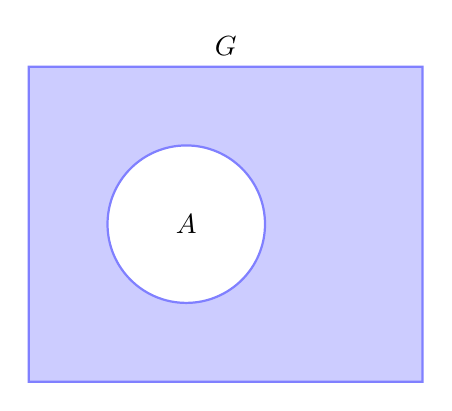
\begin{tikzpicture}
	\draw[filled] (-2,-2) rectangle (3,2) node at (-1.5,1.5) {}
	(0,0) circle (1) node {$A$};
	\node[anchor=south] at (current bounding box.north) {$G$};
\end{tikzpicture}

\subsubsection{Vereinigung}

Vereinigung $\cup$ (Mengenkonjunktion)\\
Der komplette Inhalt der einen Menge, zusammen mit dem Inhalt der anderen Menge.\\
$A := \{a,b,c\}$ , $B := \{x,y\}$\\
$A \cup B := \{x \in G | x \in A \vee x \in B\}$\\
$A \cup B = \{a,b,c,x,z\}$\\

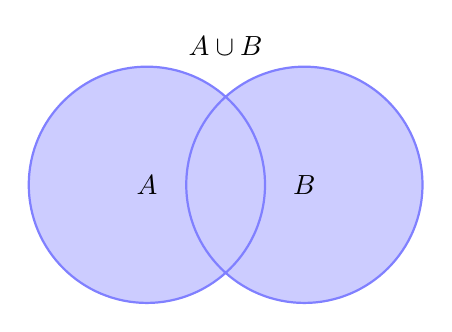
\begin{tikzpicture}
  \draw[filled] \firstcircle node {$A$}
                \secondcircle node {$B$};
  \node[anchor=south] at (current bounding box.north) {$A \cup B$};
\end{tikzpicture}

\newpage

\subsubsection{Duchschnitt}

Duchschnitt $\cap$ (Schnittmenge, Mengen Disjunktion)\\
Die Elemnte, welche A und B gemeinsam haben.\\
$A := \{a,b,c,d,e,f\}$ , $B := \{e,f\}$\\
$A \cap B := \{x \in G | x \in A \wedge x \in B\}$\\
$A \cap B = \{e,f\}$\\

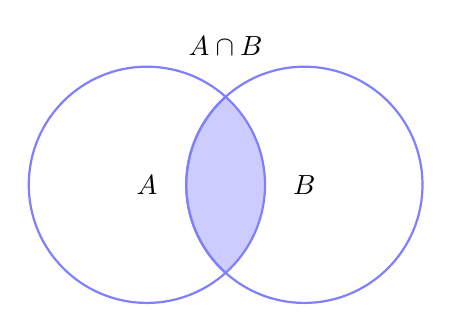
\begin{tikzpicture}
  \begin{scope}
    \clip \firstcircle;
    \fill[filled] \secondcircle;
  \end{scope}
  \draw[outline] \firstcircle node {$A$};
  \draw[outline] \secondcircle node {$B$};
  \node[anchor=south] at (current bounding box.north) {$A \cap B$};
\end{tikzpicture}

\subsubsection{Differenz}

Differenz $\not$ \hspace{2mm}(Mengen differenz)\\
Alle Elemente in A, welche nicht in B vorkommen.\\
$A := \{a,b,c,d,e,f\}$ , $B := \{e,f,g,h\}$\\
$A \setminus B := \{x \in G | (x \in A \wedge x \notin B)\}$\\
$A \setminus B = \{a,b,c,d\}$\\

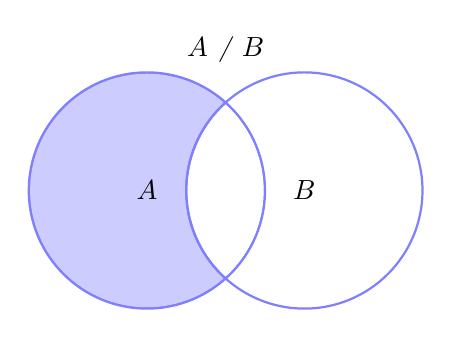
\begin{tikzpicture}
  \begin{scope}
      \clip \firstcircle;
      \draw[filled, even odd rule] \firstcircle node {$A$}
                                   \secondcircle;
  \end{scope}
  \draw[outline] \firstcircle
                 \secondcircle node {$B$};
  \node[anchor=south] at (current bounding box.north) {$A \not$ \hspace{1mm} $B$};
\end{tikzpicture}

\newpage

\subsubsection{Symmetrische Differenz}

Symmetrische Differenz $\triangle$\\
Alle Elemente in A, welche nicht in B vorkommen, und alle Elemente in B, welche nicht in A vorkommen.\\
$A := \{a,b,c,d,e,f\}$ , $B := \{e,f,g,h\}$\\
$A \triangle B := \{x \in G | (x \in A \wedge x \notin B) \vee (x \in B \wedge x \notin A)\}$\\
$A \triangle B = \{a,b,c,d,g,h\}$\\

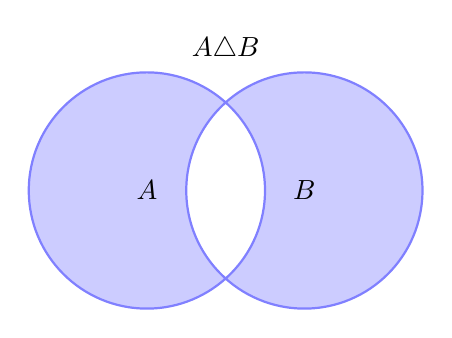
\begin{tikzpicture}
  \draw[filled, even odd rule] \firstcircle node {$A$}
                               \secondcircle node{$B$};
  \node[anchor=south] at (current bounding box.north) {$A \triangle B$};
\end{tikzpicture}

\subsubsection{Komplement}

Komplement $\overline{\rm A}$\\
Alles ausser A\\
$A := \{1,2,3,4,5\}$ , $G := \mathbb{N}$\\
$\overline{\rm A} := \{x \in G | (x \notin A\} = G \setminus A$\\
$\overline{\rm A} = \{6,7,8,9,10,...\}$\\

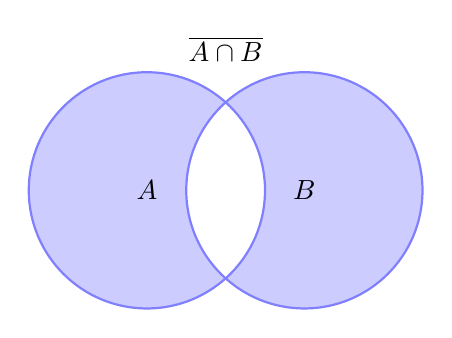
\begin{tikzpicture}
  \draw[filled, even odd rule] \firstcircle node {$A$}
                               \secondcircle node{$B$};
  \node[anchor=south] at (current bounding box.north) {$\overline{A \cap B}$};
\end{tikzpicture}

\newpage

\subsubsection{Kartesisches Produkt}

Kartesisches Produkt $\times$ (Mengenprodukt)\\
Alle Elemente von A "Multipliziert" mit allen Elementen der Menge B.\\
$A := \{1,2\}$ , $B := \{3,4\}$\\
$A \times B := \{(x,y) | x \in A \wedge y \in B\}$\\
$A \times B = \{(1,3),(1,4),(2,3),(2,4)\}$\\

\begin{tikzpicture}[
	vec/.style={thick,(-)},
 ]
	% picture commands
	\coordinate (A) at (3,0);
	\coordinate (B) at (0,-2);
	\coordinate (cross prod) at (1,3);
	\def\tick{0.1}
	\draw [->] (-1,0) -- (6,0) node [below] {$G_1$};
	\draw [->] (0,-1) -- (0,4) node [left]  {$G_2$};

	\draw [vec] (1,-0.2) -- ++(A) node [midway,below] {$A$};
	\draw [vec] (-0.2,3) -- ++(B) node [midway,left]  {$B$};

	\fill [filled] (cross prod) rectangle ++($(A)+(B)$);

	\draw node at (2.4,2) {$A \times B$};

 \end{tikzpicture}

\subsection{Bindungsstärke}

Mengenoperationen können zu längeren logischen Ausdrücken verknüpft werden.\\

Dabei gilt die folgende Bindungsstärke:

\begin{enumerate}
  \item $( )$ \hspace{7.8mm} Klammern
  \item $\overline{\rm A}$ \hspace{8mm} Komplement
  \item $\bigcap$, $\bigcup$ ($\bigcup \limits_{k=1}^n$, $\bigcap \limits_{k=1}^n$) \hspace{1mm} Vereinigung \& Durchschnitt
  \item $\cap$, $\cup$, $\setminus$, $\triangle$, $\overline{\rm A}$, $\times$ \hspace{1mm} Vereinigung \& Durchschnitt \& Differenz \& Symmetrische Differenz \& Komplement \& Kartesisches Produkt
\end{enumerate}

\newpage

\subsection{Gesetze der Mengenalgebra}

Die einzige notwendige Operatione ist das Elementenprädikat $\in$ oder $\notin$.\\
Alles andere kann durch Operatoren der Prädikatenlogik eingeführt werden.\\
Gründe für das Rechnen mit Mengen is die Möglichkeit einfache Gleichheit zu testen. Grosse und komplizierte Ausdrücke lassen sich unterteilen und vereinfachen.\\
Aussagelogik und Mengentheorie unterscheiden sich im Kontext.\\

Elementare Rechenregel:\\
\def\arraystretch{1.5}
\begin{table}[ht]
\begin{tabular}[t]{ll}
\hline
Name/Stichwort: & Regel/Gesetz:\\
\hline
  Idempotenzgesetze &
  $A \cap A = A$\\
  Kommutativgesetze &
  $A \cap B = B \cap A$ \hspace{31mm} $A \cup B = B \cup A$\\
  Identitätsgesetze &
  $A \cap G = A$ \hspace{37.5mm} $A \cup \emptyset = A$\\
  &
  $A \cap \emptyset = \emptyset$ \hspace{39mm} $A \cup G = G$\\
  Assoziativgesetze &
  $(A \cap B) \cap C = A \cap (B \cap C)$
  \hspace{11.5mm}
  $(A \cup B) \cup C = A \cup (B \cup C)$\\
  Absorptionsgesetze &
  $A \cap (A \cup B) = A$ \hspace{28mm} $A \cup (A \cap B) = A$\\
  Distributivgesetze &
  $A \cap (B \cup C) = (A \cap B) \cup ( A \cap C)$\\
  De Morgan Gesetze &
  $\overline{\rm (A \cap B)} = \overline{A} \cup \overline{B}$\\
  Komplement Gesetze &
  $A \cap \overline{A} = \emptyset$ \hspace{39mm} $A \cup \overline{A} = G$\\
  &
  $\overline{\overline{A}} = A$\\
  &
  $\overline{G} = \emptyset$\\
  &
  $\overline{\emptyset} = G$\\
  Teilmengenbeziehungen &
  $A \subseteq B \Rightarrow ( A \cap B = A)$ \hspace{20mm} $A \subseteq B \Rightarrow (A \cup B = B)$\\
  &
  $(A \subseteq B) \wedge (B \subseteq C) \Rightarrow (A \subseteq C)$\\
\hline
\end{tabular}
\end{table}

$A \triangle B$ lässt sich auch darstellen als $(A \setminus B) \cup (B \setminus A)$\\

\subsubsection{Partition einer Menge}

\begin{itemize}
  \item Eine Menge A kann viele und verschiedene Teilmengen haben.
  \item Diese kann man wieder zu Mengen zusammenfassen.
  \item Ein ganz besonders hilfreicher Typ von Mengensystem.
  \item Erlauft den Begriff der Paarung und damt den Vergleich der Mächtigkeiten, auch von unendlichen Mengen.
\end{itemize}

\begin{align}
\fbox{\begin{minipage}{11.8cm}
  \textbf{Beispiel}: 
  Eine Beispiel einer Partition $\mathbb{N}_{10}$:\\
  \\
  $\mathbb{N}_{10} := \{0,1,2,3,4,5,6,7,8,9,10\}$\\
  $S := \{\{1\},\{0,2,4,6,10\},\{3,6,9\},\{5,7\}\}$\\
  \\
  Es ist jedes Element enthalten.\\
  In den Teilmengen gibt es keine Überschneidungen.
\end{minipage}}
\end{align}

\textbf{Anwendung}:\\
\\
Die Untersuchung einer Menge kann deutlich vereinfacht werden.\\
z.B. lässt sich $\mathbb{N}$ in gerade und ungerade Zahlen trennen.\\

Die Anzahl Partitionen einer Menge M mit n Elementen lässt sich durch die sogenannte "Bell'sche Zahl" $B_n$ angeben.\\

\begin{table}[ht]
  \begin{tabular}{c|c|c|c|c|c}
    Mächtigkeit der Menge n = & 2 & 4 & 6 & 10 & 16 \\ \hline
    Bell'sche Zahl (anz. Partitionen) $B_n$ = & 2 & 15 & 203 & 115'975 & 10'480'142'147 \\
  \end{tabular}
  \quad
\end{table}

\subsection{Unendlichkeit von Mengen}

Die Fragestellung die es zu klähren gillt:\\
\\
Lassen sich kardinalitäten von unendlichen Mengen vergleichen? Ja!\\
Gibt es verschiedene Unendlichkeiten? Ja!\\

\subsubsection{Paarung zweier Mengen}

Sei: $A := \{1,2,3,4\}$ und $B := \{a,b,c,d\}$\\
Teilmenge T1 := $\{(1,c),(2,b),(3,d),(4,a)\}$ ist eine Paarung von Menge A und B\\
Teilmenge T2 := $\{(1,d),(2,c),(3,a),(4,ab)\}$ ist eine andere Paarung von Menge A und B\\
Teilmenge T3 := $\{(1,d),(2,a),(3,c)\}$ ist keine Paarung von A und B. (4 und b fehlen).\\

Zwei Mengen A und B (endlich oder unendlich) haben die gleiche Mächtigkeit 
$|A| = |B|$, wenn es eine Paarung von A und B gibt.

\subsubsection{Nummering, Ordnung}

Wenn es eine Paarung von $\mathbb{N}$ mit einer Menge A gibt, so kann man diese 
Paarung als Nummerierung von A auffassen.\\
\\
z.B.: Menge $A := \{a*,a^2, a_3\}$\\
ergibt: $\{(0,a*),(1,a^2),(2,a_3)\}$\\
\\
Wir nennen das n des Elements auch die Ordnung dieses Elements oder den Index von.\\
\\
Mit Hilfe der Paarung könen wir auch eine andere, gleichwertige Definition der 
unendlichen Mengen formulieren:\\
Eine Menge A heisst unendlich, wenn es eine echte Teilmenge $T \subsetneq A$ 
gibt, sodass A und T eine Paarung sind.\\
Beispiel: $\mathbb{N}$ ist unendlich wegen der Paarung von A und B.\\
$A := \mathbb{N}$, $B := \{1,2,3,4,5,6,...\}$\\
Paarung = $\{(0,1),(1,2),(2,3),(3,4),...\}$\\
Weil B eine echte Teilmenge von $\mathbb{N}$ ist (0 fehlt in B).\\
\\
Eine Menge heisst abzählbar unendlich, wenn es eine Paarung mit $\mathbb{N}$ 
gibt, d.h. wenn sie gleichmächtig wie $\mathbb{N}$ ist.
Endliche und abzählbar unendliche Mengen nennen wir zusammen auch abzählbare 
Mengen.

\begin{align}
\fbox{\begin{minipage}{11.8cm}
  \textbf{Beispiel}: $\mathbb{Z}^-$, $\mathbb{Z}^+$, $\mathbb{Z}$\\
  Die Menge $\mathbb{N}_g$ der geraden und die Menge $\mathbb{N}_u$ der 
  ungeraden Zahlen sind alle gleichmächtig, also abzählbar unendlich.
\end{minipage}}
\end{align}

Eine Menge heisst überabzählbar unendlich, wenn sie unendlich ist und nicht 
abzählbar (d.h. "mächtiger" als $\mathbb{N}$).

\begin{align}
\fbox{\begin{minipage}{11.8cm}
  \textbf{Beispiel}: $\mathbb{R}$ ist überabzählbar unendlich 
  $|\mathbb{N}| < |\mathbb{R}|$.
\end{minipage}}
\end{align}

Unendliche Mengen verhalten sich bedeuntend unintuitiver als endliche Mengen.\\

Die Kontinuumhypothesis beschäftigt sich mit der Frage; Gibt es eine Menge A zwischen $|\mathbb{N}| < |A| < \mathbb{R}$?\\
Die Antwort ist bis heute ungeklährt und wird deshalb verneint, also es gibt keine Menge, deren Mäctigkeit dazwischen liegt.
